%==============================================================================
% Documentation (pdflatex --interaction=nonstopmode this_file.spad
% Note: ensure that the code above is between \iffalse ... \fi.
%==============================================================================
\documentclass[12pt,a4paper]{article}
\usepackage[utf8]{inputenc}
\usepackage[english]{babel}
\usepackage{amsmath}
\usepackage{amsfonts}
\usepackage{amssymb}
\usepackage{makeidx}
\usepackage{graphicx}
\usepackage{listings}
\usepackage{color}
\usepackage{epstopdf}

\definecolor{dkgreen}{rgb}{0,0.6,0}
\definecolor{gray}{rgb}{0.5,0.5,0.5}
\definecolor{mauve}{rgb}{0.58,0,0.82}
\definecolor{orange}{rgb}{1.0,0.44,0}

\lstdefinelanguage{SPAD}
{keywords={if,then,else,for,in,repeat},
keywords=[2]{Fraction,Integer,Polynomial,RealClosure,Cell, Float, 
             DoubleFloat, CylindricalAlgebraicDecompositionPackage, 
             List},
keywords=[3]{cylindricalDecomposition},
keywordstyle=[2]\color{red},
keywordstyle=[3]\color{orange},
sensitive=true,%
alsoletter={\$},%
comment=[l]{--},%
string=[b]",%
string=[b]'%
}

\lstset{frame=tb,
  language=SPAD,
  aboveskip=3mm,
  belowskip=3mm,
  showstringspaces=false,
  columns=flexible,
  basicstyle={\small\ttfamily},
  numbers=none,
  numberstyle=\tiny\color{gray},
  keywordstyle=\color{blue},
  commentstyle=\color{dkgreen},
  stringstyle=\color{mauve},
  breaklines=true,
  breakatwhitespace=true,
  tabsize=3
}
\author{Kurt Pagani \\ {\tt nilqed@gmail.com}}
\date{\today}
\title{DifferentialForms \\ {\small\tt FriCAS package:DFORM \\ Version 1.2}}
%
\newcommand{\CAD}{{\tt CAD}}
\newcommand{\QE}{{\tt QE}}
\newcommand{\RR}[1]{\mathbb{R}^{#1}}
\newcommand{\QQ}[1]{\mathbb{Q}^{#1}}
\newcommand{\ZZ}[1]{\mathbb{Z}^{#1}}
\newcommand{\KK}[1]{\mathbb{K}^{#1}}
%
\begin{document}
\maketitle
%
\begin{abstract}
lorem ipsum. 
\end{abstract}
%
\section{Introduction}
The package {\tt DifferentialForms} (file: {\tt dform.spad}) builds on the
domain {\tt DeRhamComplex}. In the following section we will give a brief 
overview of the functions that are going to be implemented. The focus is 
on precise definitions of the notions, since those may be varying in the 
literature. In section (2) we will describe the exported functions and 
how they work, in section (3) some short implementation notes will be 
given and finally the last section is devoted to some examples.
%
\section{Definitions}
Let ${\cal M}$ be a n-dimensional manifold (sufficiently smooth and orientable). 
To each point $P\in{\cal M}$ there is a neighborhood which can be 
diffeomorphically mapped to some region in $\RR n$, with coordinates
\begin{displaymath}
   x_1 (P'), \ldots, x_n (P')
\end{displaymath}
for all $P' \in \mathcal{U} (P) \subset \mathcal{M}$. The tangent space
$T_{P'} (\mathcal{M})$ at the point $P'$ is a vector space that 
is spanned by the basis
\begin{displaymath}
    e_1 (P'), \ldots, e_n (P')
\end{displaymath}
which also is often denoted by 
\begin{displaymath}
   \partial_1, \ldots, \partial_n =
   \frac{\partial}{\partial x_1}, \ldots, 
   \frac{\partial}{\partial x_n}.  
\end{displaymath}
A tangent vector $v$ has the form

\begin{displaymath}
  v = \sum_{j = 1}^n v^j e_j . 
\end{displaymath}
The cotangent space $T_{P'}^{} (\mathcal{M})^{\star}$ is the vector space
of linear functionals 
\begin{displaymath}
   \alpha : T_{P'} (\mathcal{M}) \rightarrow \mathbb{R},
\end{displaymath}
spanned by the basis $e^1 (P'), \ldots, e^n (P')$
which (corresponding to the basis $\partial_j$) is also denoted by 
\begin{displaymath}
	d x^1,\ldots, d x^n. 
\end{displaymath}
The latter notation indicates the dependency on the moving
point $P'$. The dual basis is by definition comprised of those linear
functionals such that
\begin{displaymath}
  e^j (e_k) = \delta^j_k . 
\end{displaymath}
Therefore we have 
\begin{displaymath}
	\alpha (v) = \alpha \left( \sum_{j = 1}^n v^j e_j \right) =
   \sum_{j = 1}^n v^j \alpha (e_j) = \sum_{j = 1}^n v^j \alpha_j,
\end{displaymath}
where $\alpha = \sum_{j = 1}^n \alpha_j e^j$.   

\subsection{Inner product of differential forms ({\tt dot})}
Let $g_x$ be a symmetric $n \times n$ matrix which is 
nondegenerate (i.e. $\det (g_x) \neq 0$). The index $x$ indicates that 
this matrix depends on the coordinates $x_1 (P), \ldots, x_n (P)$ and 
may be varying from point to point. If this dependency is smooth (enough) 
we speak of a (pseudo-) {\it Riemannian metric} (locally). This way we 
get an isomorphism between tangent vectors and $1$-forms (aka covectors):
\begin{displaymath}
	\alpha_j = g_{j k} v^k, \hspace{1.2em} v^j = g^{j k} \alpha_j .
\end{displaymath}
Clearly, $\sum_k g^{j k} g_{k l} = \delta^j_l$, in other words 
$(g^{j k})$ is the inverse of $g$. The metric $g$ defines an 
{\it inner product} on vectors,
\begin{displaymath}
	g (v, w) = \langle v, w \rangle : = g_{i j} v^i w^j 
\end{displaymath}
and by duality also on $1$-forms:
\begin{displaymath}
	 g^{- 1} (\alpha, \beta) = \langle \alpha, \beta \rangle : = g^{i j}
   \alpha_i \beta_j . 	
\end{displaymath}
Now, this inner product is extended to arbitrary $p$-forms by
\begin{displaymath}
	  \langle \alpha_1 \wedge \ldots \wedge \alpha_p , \beta_1 \wedge
  \ldots \wedge \beta_p \rangle : = \det (\langle \alpha_i, \beta_j \rangle)
  , \hspace{1.8em} (1 \leqslant i, j \leqslant p), \label{dot}
\end{displaymath}
and linearity.
%

\subsection{ The volume form $\eta$ ({\tt volumeForm})}
The Riemannian {\it volume form} $\eta$ is (by definition) given by the 
$n$-form 
\begin{displaymath}
	 \eta = \sqrt{| \det g |} e^1 \wedge \ldots \wedge e^n = 
	 \sqrt{| \det\,g |} dx^1 \wedge \ldots \wedge d x^n . \label{vol}
\end{displaymath}
This definition makes sense because a (orientation preserving) change of
coordinates $\sqrt{\mathrm{det} g}$ transforms like the component of
a $n$-form.
%

\subsection{Hodge dual ({\tt hodgeStar})}
The {\it Hodge dual} of a differential $p$-form $\beta$ is the 
$(n - p)$-form $\star \beta$ such that
\begin{displaymath}
	 \alpha \wedge \star \beta = \langle \alpha, \beta \rangle \eta 
	 \label{hodge}
\end{displaymath}
holds, for all $p$-forms $\alpha$. The linear operator $(\star)$ is 
called the {\it Hodge star operator}. By the {\it Riesz representation
theorem} the Hodge dual is uniquely defined by the expression above.
%

\noindent
{\bf Warning:} {\it Flanders} \cite{FLAN} defines the Hodge dual by the 
equality
\begin{displaymath}
	 \lambda \wedge \mu = \langle \star \lambda, \mu \rangle \eta 
\end{displaymath}
where $\lambda$ is a $p$-form and $\mu$ a $(n-p)$-form.
This may result in different signs (actually $\star_F = s(g)\star$,
where $s(g)$ is the {\it sign} of the determinant of $g$).
 
The generally adopted definition is the one given at the beginning 
of this subsection. 

The components of $\star \beta$ are

\begin{displaymath}
	(\star \beta)_{j_1, \ldots, j_{n - p}} = \frac{1}{p!} \varepsilon_{i_1,
   \ldots, i_p, j_1, \ldots, j_{n - p}}  \sqrt{| \det g |} g^{i_1 k_1} \ldots
   g^{i_p k_p} \beta_{k_1, \ldots, k_p} 
\end{displaymath}
what is equal to
\begin{displaymath}
	 \frac{1}{p! \sqrt{| \det g |}} \varepsilon_{}^{k_1, \ldots, k_p, l_1,
   \ldots, l_{n - p}} g_{j_1 l_1} \ldots g_{j_{n - p}, l_{n - p}} \beta_{k_1,
   \ldots, k_p} .
\end{displaymath}
%

\subsection{Interior product $i_v$ ({\tt interiorProduct})}
The {\it interior product} of a vectorfield $v$ and a $p$-form $\alpha$
is a $(p-1)$-form $i_v(\alpha)$ such that
\begin{displaymath}
	 i_v (\alpha) (v_1, \ldots, v_{p - 1}) = 
	   \alpha (v, v_1, \ldots, v_{p - 1})
\end{displaymath}
holds for all vectorfields $`v_1, \ldots, v_{p - 1}$. Therefore, the 
components of $i_v (\alpha)$ are calculated to
\begin{displaymath}
	 i_v (\alpha)_{j_1, \ldots, j_{p - 1}} = 
	 v^j \alpha_{j, j_1, \ldots, j_{p -1}}.
\end{displaymath}
One can express the interior product by using the $\star$-operator. 
Let $\alpha$ be the $1$-form defined by the equation 
\begin{displaymath}
	 \alpha (w) = g (v, w), \forall w. 
\end{displaymath}
This means in components: $\alpha_j = g_{j k} v^k$, 
thus we have
\begin{displaymath}
	i_v (\beta) = (-)^{p - 1} \star^{- 1} (\alpha \wedge \star \beta) .
\end{displaymath}
Clearly, the interior product is independent of any metric, whereas the 
Hodge operator is {\bf not}! So, usually one should not use the Hodge 
operator to compute the interior product.

We will use the fact that the interior product is an {\it antiderivation},
which will allow a recursive implementation.
%

\subsection{The Lie derivative $\mathcal{L}_v$ ({\tt lieDerivative})} 
The {\it Lie derivative} with respect to a vector field $v$ can be 
calculated (and defined) using {\it Cartan's} formula:
\begin{displaymath}
	\mathcal{L}_v \alpha = d i_v (\alpha) + i_v (d \alpha).
\end{displaymath}

There are other ways to define $\mathcal{L}_v \alpha$, however, 
it is convenient to compute it this way when $d$ and $i_v$ are 
already at hand.
%

\subsection{The CoDifferential $\delta$ ({\tt codifferential})}
The {\it codifferential} $\delta$ acting on a $p$-form is defined 
as follows:
\begin{displaymath}
	 \delta = (-1)^{n(p-1)+1}\,s(g) \star\,d\,\star
\end{displaymath}
where $g$ is the metric and $s(g)$ is related to the 
{\it signature} of $s(g)$ as described next.
%

\subsection{The sign of a metric  $s(g)$ ({\tt s})}
The signature of a metric $g$ is defined as the difference of
the number of positive ($p$) and negative ($q$) eigenvalues, i.e:
\begin{displaymath}
	\mathrm{signature(g)} = p - q
\end{displaymath}
and the {\it sign} function $s$ is defined as
\begin{displaymath}
	s(g) = (-1)^{\frac{n -\mathrm{signature(g)}}{2}} 
\end{displaymath}
Since we always assume that $g$ is non-degenerate, we have 
$p+q=n$, and consequently
\begin{displaymath}
	s(g) = (-1)^{q} = \mathrm{sign}\, \mathrm{det}(g)
\end{displaymath}
%

\subsection{ The inverse Hodge star $\star^{-1}$ ({\tt invHodgeStar})}
Applying the Hodge star operator on a $p$-form twice we get
the identity map up to sign:
\begin{displaymath}
	\star\circ\star\, \omega_p = (-1)^{p(n-p)}\,s(g)\,\omega_p.
\end{displaymath}
Therefore
\begin{displaymath}
	\star^{-1}\,\omega_p = (-1)^{p(n-p)}\,s(g)\,\star\omega_p. 
\end{displaymath}
%

\subsection{The Hodge-Laplacian $\Delta_g$ ({\tt hodgeLaplacian})}
The {\it Hodge-Laplacian}, also known as {\it Laplace-de Rham operator} 
is defined on any manifold equipped with a (pseudo-) Riemannian
metric $g$ and is defined by
\begin{displaymath}
	\Delta_g = d\circ\delta + \delta\circ d
\end{displaymath}

Note that in the {\it Euclidean} case $\Delta_g = - \Delta$, where
latter is the ordinary {\it Laplacian}.
%
%
%
\section{Export}
%
\subsection{Package Details}
%

\begin{tabular}{|l|l|}
   \hline 
   {\bf Package Name:} & {\tt DifferentialForms} \\ 
   \hline 
   {\bf Abbreviation:} & {\tt DFORM} \\ 
   \hline 
   {\bf Source file(s):} & {\tt dform.spad} \\ 
   \hline 
   {\bf Dependent on} & {\tt DeRhamComplex (DERHAM)} \\ 
   \hline 
   \end{tabular}    
%
\begin{lstlisting}
    DifferentialForms(R,v) 
    
    R: Join(Ring,Comparable)     -- e.g. Integer
    v: List Symbol               -- e.g. [x,y,z] or [x[0],x[1],x[2]]

    X ==> Expression R           -- function Ring   
\end{lstlisting}
%
For the examples that follow we will choose {\tt R=Integer}, 
\begin{verbatim}
    v=[x[0],x[1],x[2],x[3]]},
\end{verbatim}
and the abbreviation {\tt M:=DFORM(R,v)}. Recall that indices of lists
and vectors in FriCAS start with $1$, so one has to be careful:
\begin{verbatim}
    v.1  -->  x[0].
\end{verbatim}
%

\subsection{The metric $g$}
Some functions expect the metric $g$ as a parameter. Generally this
will be provided by an invertible square matrix 
{\tt g:SquareMatrix(\#v,X)}. 
In the sequel we will choose the Minkowski metric:
%
\begin{lstlisting}    
    g := diagonalMatrix([-1,1,1,1])@SquareMatrix(4,Integer)
\end{lstlisting}   

\begin{displaymath}
	 \left[
  \begin{array}{cccc}
  -1 & 0 & 0 & 0 \\
  0 & 1 & 0 & 0 \\
  0 & 0 & 1 & 0 \\
  0 & 0 & 0 & 1
  \end{array}
  \right]
\end{displaymath}

 
  
%:sub:`Type: SquareMatrix(4,Integer)`


%
%\begin{figure}[!htb]
%\centering
%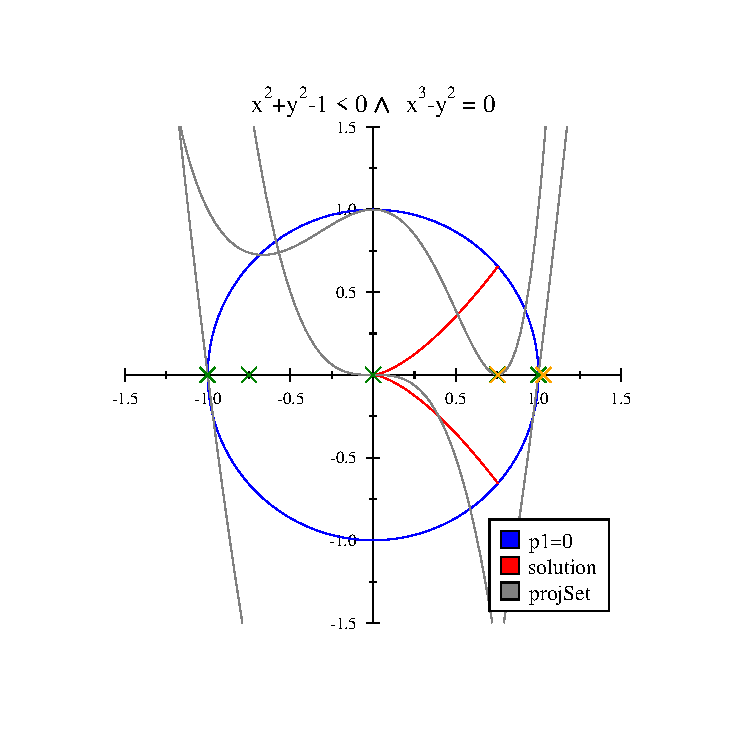
\includegraphics[scale=1.0]{cad1.eps}
%\caption{Example 1.}
%\label{fig:cad1}
%\end{figure}
% 
\begin{thebibliography}{1}
%
\bibitem{MTAA} Ralph Abraham, Jerrold E.Marsden and Tudor Ratiu.Manifolds, 
       {\em Tensor Analysis, and Applications}. Springer,
       Auflage: 2nd Corrected ed. 1988. Corr. 2nd printing 1993 edition.
%       
\bibitem{CART} Henri Cartan. {\em Differential Forms}. Dover Pubn Inc.
%
\bibitem{GMT} Herbert Federer. {\em Geometric Measure Theory}. Springer, 
       Reprint of the 1st ed. Berlin, Heidelberg, New York 1969 edition.
%
\bibitem{FLAN} Harley Flanders, {\em Differential Forms with Applications to 
       the Physical Sciences}. Dover Pubn Inc, Revised. edition.
%
\bibitem{QYBEQ} L. A. Lambe and D. E. Radford. {\em Introduction to the 
       Quantum Yang-Baxter Equation and Quantum Groups:An Algebraic Approach}.
       Springer, 1997 edition.
%
\bibitem{PMA} Walter Rudin and RudinWalter.{\em Principles of Mathematical
       Analysis}. McGraw Hill Book Co, Revised. edition.
%
\bibitem{GIT} Hassler Whitney. {\em Geometric Integration Theory}, 
       Princeton Mathematical Series, No. 21. Literary Licensing, LLC.
\end{thebibliography}
%
\end{document}
% -----------------------------------------------------------------------------
% END DOCUMENTATION
% -----------------------------------------------------------------------------
